% This file (dissertation-main.tex) is the main file for a dissertation.
\documentclass {udthesis}
% preamble

% Include graphicx package for the example image used
% Use LaTeX->PDF if including graphics such as .jpg, .png or .pdf.
% Use LaTeX->PS->PDF if including graphics such as .ps or .eps
% Best practice to not specify the file extension for included images,
% so when LaTeX is building it will look for the appropriate image type.
\usepackage{graphicx}
\usepackage[acronym]{glossaries}
\usepackage{enumitem}
\usepackage{amsmath}
\usepackage{caption}
\usepackage{subcaption}
\usepackage{url}
\usepackage{booktabs}
\usepackage{tikz}
\usetikzlibrary{matrix,shapes,arrows,positioning,chains}

%%%%%%%%%%%%%%%%%%%%%%%%%%%%%%%%%%%%%%%%%%%%%%%%%%%%%%%%%%%%
% List of acronyms
%%%%%%%%%%%%%%%%%%%%%%%%%%%%%%%%%%%%%%%%%%%%%%%%%%%%%%%%%%%%

\newacronym{auv}{AUV}{Autonomous Underwater Vehicle}
\newacronym{rov}{ROV}{Remotely Operated Vehicle}
\newacronym{hov}{HOV}{Human Operated Vehicle}
\newacronym{api}{API}{Application Program Interface}
\newacronym{dyi}{DYI}{Do It Yourself}
\newacronym{ros}{ROS}{Robot Operating System}
\newacronym{dof}{DOF}{Degree of Freedom}
\newacronym{imu}{IMU}{Inertial Measurement Unit}
\newacronym{cad}{CAD}{Computer Aided Design}
\newacronym{lipo}{LiPo}{Lithium Polymer}
\newacronym{tcp}{TCP}{Transmission Control Protocol}
\newacronym{acp}{AC}{Alternating Current}
\newacronym{dcp}{DC}{DIrect Current}
\newacronym{fps}{FPS}{Frames Per Second}
\newacronym{ar}{AR}{Augmented Reality}
\newacronym{rst}{RST}{Rotation, Scaling and Translation}
\newacronym{fov}{FOV}{Field of View}



\makeglossaries
\graphicspath{{fig/}}

\begin{document}

%=========================================================================================
% CoopROV section

\chapter{CoopROV: Low cost underwater remotely operated vehicle}
\label{chap:cooprov}

%=========================================================================================
% Outline
\section{Outline}

The developed multi-image object recognition theory can be validated using an easily accessible 
open-source robot.

\begin{enumerate}[label=Section \arabic*:, start=0]
\item Intro

\item Commercially available underwater robots are expensive and provide limited flexibility for incorporation of new sensors and custom controllers.

\item CoopROV based off of the open-source underwater platform openROV, marries the low cost hardware design with seamless integration to ROS for easy application development.

\item An underwater experimental setup in a water tank was designed to collect underwater image data.

\item IMU, depth sensor, stereo camera and AR Tags were used to localize CoopROV.

\item The multi-image object recognition approach was validated using image data gathered from CoopROV.

\end{enumerate}

%========================================================================================

\section{Introduction}

Field experiments related to underwater object recognition require a submersible robot with appropriate sensing and control payload to navigate through points of interest and capture necessary data through sensors. Depending on the level of manual intervention involved to guide the vehicle, an underwater vehicle, can be classified as an \gls{auv}, a \gls{rov} or a \gls{hov}. \gls{auv}s navigate autonomously with minimal to no manual intervention. Both \gls{rov}s and \gls{hov}s are piloted by humans, with the difference being that the human operator is within the vehicle in an \gls{hov}, whereas in the \gls{rov} the human operator controls the vehicle from a remote location. Commercially available underwater vehicles come with wide range of capabilities in terms of sensing and operational depths. The sensing package or the type of vehicle required is dictated by the objective of the science experiment and its requirements. For validation and fine-tuning of the underwater object recognition algorithms like the 
multi-layered scallop recognition (Chapter~\ref{chap:scallop_recog}) and the multi-view object recognition (Chapter~\ref{chap:distdes}), an underwater vehicle that can navigate to specific points and collect image data of underwater targets is needed. With these requirements in mind, a low-cost underwater research vehicle named CoopROV was developed. CoopROV is a \gls{rov}-class vehicle that is equipped with several sensors for data collection, and also has the capability to incorporate any customized controller.

\section{Commercial Submersible Robots}

Commercially available robots are expensive and often provide minimal access to their legacy controllers and software. Most commercial \gls{rov}s come with a graphical interface and joystick. \gls{auv}s come with an interface to allow the user to predefine the robot trajectory through a series of geo-tagged waypoints before deployment. Once deployed, the \gls{auv} tracks the specified trajectory. Such manufacturer interfaces do not provide considerable freedom to modify the core software running on the robot. For instance if someone wants to use their own controller, it becomes problematic to implement it without manufacturer supported software \gls{api}s. Cost is another factor that limits accessibility to commercial underwater robots. A relatively small \gls{rov} like the videoray \cite{videoray} with a footprint of $14.75\times 11.4\times 8.75 \,(L\times W\times H \text{ in inches})$ and a sensor package comprising a camera, gyros, accelerometers, compass, depth and temperature sensors can cost 
over 25\,000 dollars. Bigger \gls{rov}s like the Outland ROV~\cite{outlandrov} can cost upwards of 75\,000 dollars with the cost here being chiefly determined by the sophistication of the on board sensing capabilities. Despite the high cost and minimal flexibility for customer modifications, the primary advantage of these commercial solutions is their well tested hardware that is resilient to harsh conditions that are characteristic to the marine environments.

The other league of underwater robotic solutions come in form of low-cost \gls{dyi} style robots like the OpenROV \cite{openrov} and the Fathom One~\cite{fathomrov}. Such solutions offer a lot of potential for custom hardware and software modifications. However being small-scale development projects, the associated hardware in these cases is not well tested and can be prone to failures (e.g. water leaks). The capability of these systems to withstand the harsh conditions of a marine environment may be limited. In terms of software, the source code is often available and comes with an open-source license (as in the case of OpenROV). However such software often does not come with \gls{api}s to encourage users to extend or modify the capabilities of the robot. Additionally, the limited documentation available makes the task of directly modifying the source code cumbersome. Since the focus of most of these \gls{dyi} projects are to offer low-cost options that primarily enable hobbyists to explore underwater, a 
teleoperation 
interface and access to a camera feed from the robot typically suffices. For researchers that may have very specialized interests, an ideal robotic solution should offer finer control of the hardware and software with options to easily extend the base capabilities of the system.

There are two primary requirements for a professionally developed robotic solution that is intended for research. The first is the need for a tough exterior shell that can hold up against high values of water pressure which is common with deep sea operation. This exterior shell should also be resilient to water leaks and at the same time offer the ability to retrofit sensors. The second requirement is for the robotic system to offer a well built software interface with \gls{api}s that allows researchers to extend the capabilities of the system. It will be beneficial if the software \gls{api}s adhere to popular robotics research architectures like the \gls{ros}~\cite{ros} or \gls{moos}~\cite{moos}. A robot with \gls{ros}-support will greatly enhance the versatility of the robot by allowing access to a plethora of existing software tools. Furthermore, software development based on open-source tools like \gls{ros} can be supported by an active base of researchers that can provide feedback, 
tips and advice. Currently the underwater research community lacks a variety of low-cost submersible 
robotic platforms with resilient hardware design and well-engineered software.

\section{CoopROV}

The chief requirements that led to the design of CoopROV was the need for a low-cost submersible robotic platform that can serve as a test-bed for computer vision and control algorithms. Before the effort to build CoopROV was initiated, existing solutions were evaluated. Commercial robotic solutions like the Videoray were clearly outside the budget of this research project. OpenROV 2.5~\cite{openrov}, the first version of OpenROV, was a good candidate primarily due to it sub-1000 dollar price tag. The original OpenROV design came with a beaglebone and browser based graphical user interface that used node.js \cite{nodejs} in the backend to drive the robot. However, multiple tests revealed that the water proofing design and electronics package had several glitches making it unsuitable for deployment in its original configuration. Furthermore, most of the algorithm development till that point was in \gls{ros}, hence \gls{ros} support was one of the 
preferred requirements for the submersible robot. The initial experimental evaluation of OpenROV provided useful insights into the core components and associated problems that need to be tackled to design a submersible robot. The design of CoopROV was initiated to address the shortcomings of OpenROV's hardware in terms of waterproofing and electronics. Additional features of the target design was to allow easy interfacing of new sensors along with full \gls{ros} software support for sensors and actuators.

In the current stage of development, CoopROV shows some resemblance to OpenROV as both of them share the same frame and actuators. However, all electronics, power-supply and sensors in CoopROV have diverged completely from OpenROV 2.5. Two views of CoopROV a frontal view and its appearance when deployed in a test tank are shown in Figure~\ref{fig:cooprov}.
%
\begin{figure}
  \centering
  \begin{subfigure}[]{0.45\textwidth}
      \includegraphics[width=\textwidth]{cooprov_front}
      \label{fig:cooprov_front}
  \end{subfigure}
  \begin{subfigure}[]{0.45\textwidth}
      \includegraphics[width=\textwidth]{cooprov_top}
      \label{subfig:cooprov_top}
  \end{subfigure}
  \caption[CoopROV]{CoopROV shown in two different views}
  \label{fig:cooprov}
\end{figure} 

\subsection{System Overview}

CoopROV is a \gls{rov}-class submersible that is connected to a surface station through a tether. The surface station is a laptop computer. CoopROV and its surface station are connected by an ethernet interface and run a distributed \gls{ros} system. In teleoperation mode, a joystick controller connected to the surface station can drive the robot. The joystick controller can actuate the 3 thrusters (two at the back and one on top) offering the robot a 6-\gls{dof} motion capability. This data flow between the different system components is graphically illustrated in Figure~\ref{fig:cooprov_dataflow}. The computing on the robot is handled by a RaspberryPi~\cite{raspberrypi} and Arduino Mega~\cite{arduino}. The sensor package includes a stereo camera, a 9-\gls{dof} \gls{imu}, depth, temperature and voltage sensors. The robot is powered by two sets of \gls{lipo} batteries which can provide up to an hour of run time. For a brief list of CoopROV specifications see Table~\ref{tab:cooprov_specs}. A more detailed 
account of 
different subsystems comprising hardware, electronics, software, sensors and power supply is given in the following sections.
%
\begin{table}	
  \begin{tabular}{lll} 
  \toprule
  Weight			&7 Kg\\
  Dimensions (L x W x H)	&0.30 x 0.28 x 0.39 m\\
  Run time			&1 hour\\
  Sensors			&Minoru stereo 3D webcam \\
				&LIS3MDL 3-axis magnetometer	\\
				&LSM6DS33 3-axis accelerometer and gyro\\
				&MS5803 pressure and temperature sensor\\
				&\gls{lipo} tester voltage sensor\\
  \bottomrule
  \end{tabular}
  \caption{CoopROV Specifications}
  \label{tab:cooprov_specs}
\end{table}
  
\begin{figure} 
  \centering
  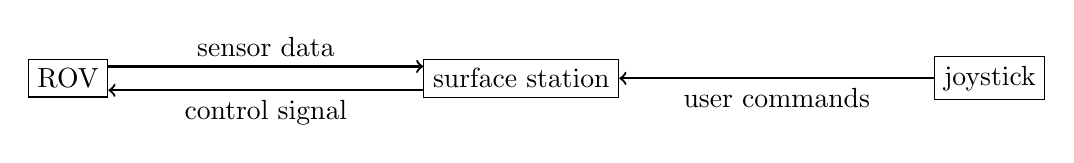
\begin{tikzpicture}[node distance = 4cm, auto]
      % Place nodes
      \node [rectangle, draw] (rov) {ROV};
      \node [right= of rov, rectangle, draw] (ss) {surface station};
      \node [right= of ss, rectangle, draw] (joy) {joystick};
      % Draw edges
      \path [->, thick] ([yshift=1ex]rov.east) edge node {sensor data} ([yshift=1ex]ss.west);
      \path [->, thick] ([yshift=-1ex]ss.west) edge node {control signal} ([yshift=-1ex]rov.east);
      \path [->, thick] (joy) edge node {user commands} (ss);
  \end{tikzpicture}
\caption[CoopROV data-flow diagram]{Block diagram of high-level data flow between different components in CoopROV}
\label{fig:cooprov_dataflow}
\end{figure}


\subsection{Hardware}

The exterior shell of CoopROV is composed of an acrylic frame that holds all housing tubes together. There are 3 housing tubes in total: an electronics tube, a connector tube and a battery tube. A \gls{cad} model of CoopROV in Figure~\ref{fig:cooprov_cad} illustrates the position of the housing tubes on the CoopROV frame. The electronics tube is a long transparent acrylic tube that holds all sensors and most electronics of the robot. The connector housing tube is a relatively short transparent acrylic tube with a molex connector plug inside it. This connector tube serves as a water proof connector plug that allows to change the sensor package by swapping out the electronics tube. The battery tube is a PVC pipe that holds 11.1 V Li Ion batteries. The clips and clamps that hold the tubes in place were made out of 3D-printed plastic parts. One big design improvement over OpenROV is the water proof seals. The waterproof seals comprise a delrin end cap with an O-ring seal along with 3 threaded rods to maintain 
the tension between the end caps and the acrylic tube. 
%
\begin{figure}	
    \centering
    \begin{subfigure}[]{0.33\textwidth}
        \centering
        \includegraphics[width=0.95\linewidth]{cooprov_frontview}
        \caption{Front view}
        \label{fig:cooprov_frontview}
    \end{subfigure}%
    \begin{subfigure}[]{0.33\textwidth}
        \centering
        \includegraphics[width=0.95\linewidth]{cooprov_sideview}
        \caption{Side view}
        \label{fig:cooprov_sideview}
    \end{subfigure}%
    \begin{subfigure}[]{0.33\textwidth}
        \centering
        \includegraphics[width=0.95\linewidth]{cooprov_isobackview}
        \caption{Isometric view (back)}
        \label{cooprov_isobackview}
    \end{subfigure}
    \begin{subfigure}[]{0.7\textwidth}
        \centering
        \includegraphics[width=0.95\linewidth]{cooprov_labels}
        \caption{Isometric view (front)}
        \label{cooprov_labels}
    \end{subfigure}
    \caption[CoopROV CAD model]{Different views of the CoopROV \gls{cad} model with some labeled parts}
    \label{fig:cooprov_cad}
\end{figure}

\subsection{Electronics}

The electronic components inside the electronics tube are responsible for controlling the thrusters and relaying the sensor data back to the surface station. The RaspberryPi and the surface station together constitute a distributed \gls{ros} system. For communication purposes, a \gls{tcp} link is established between the RaspberryPi and the surface station via the tether cable. The Arduino is connected to the RaspberryPi via the serial bridge and behaves like a node on the \gls{ros} system. The Arduino logs the data from the depth sensor and the \gls{imu}. Additionally, the arduino is also responsible for translating the motor commands into signals for the motor driver. The stereo camera's image data acquisition is directly handled through a usb interface on the RaspberryPi.

There are two parallel data streams. One enables the flow of control commands throughout the system and other handles the data being logged from the various sensors. The control commands from the joystick flow through the surface station and RaspberryPi to reach the Arduino. The Arduino translates these motor velocity commands in to \gls{pwm} signals, that enable the motor driver to run the propellers. The sensor data logged by the Arduino and RaspberryPi are served to other nodes on the \gls{ros} system through a \emph{publish-subscribe} architecture. The block diagram in Figure~\ref{fig:cooprov_electronics} provides a graphical overview of the connections between the major electronic components on CoopROV. It is important to note that only one motor and motor driver are shown in Figure~\ref{fig:cooprov_electronics}, but in the actual system, there are 3 motors with dedicated motor drivers. Figure~\ref{fig:cooprov_electronics} also shows the two power supplies in the system. More details 
on the power supply components can be found in next section.

\begin{figure}
\centering
% Define block styles
\tikzset{
    block/.style={
        rectangle,
        draw,
        text width=10em,
        text centered,
        rounded corners
    },
    rectangle_connector/.style={
        to path={(\tikztostart) -- ++(#1,0pt) \tikztonodes |- (\tikztotarget) },
        pos=0.5
    },
    rectangle connector/.default=-2cm,
}
  \begin{tikzpicture}[auto]
      % Place nodes
      \node [rectangle, draw] (ps5) {Power supply 5V};
      \node [above right= of ps5, rectangle, draw] (rpi) {RaspberryPi};
      \node [below= of rpi, rectangle, draw] (ard) {Arduino};
      \node [right= of rpi, rectangle, draw] (stereo) {Stereo camera};
      \node [above right= 0.01cm and 1.4cm of ard, rectangle, draw] (depth) {Depth sensor};
      \node [below right= 0.01cm and 1.4cm of ard, rectangle, draw] (imu) {IMU};
      \node [below= of ard, rectangle, draw] (motdr) {Motor driver};
      \node [below= of motdr, rectangle, draw] (ps11) {Power supply 11.1V};
      \node [right= of motdr, rectangle, draw] (mot) {Thruster};

      % Draw edges
      \draw [rectangle_connector=2cm,->,thick] (ps5) to node {} (rpi);
      \draw [rectangle_connector=2cm,->,thick] (ps5) to node {} (motdr);
      \draw [rectangle_connector=1.5cm,<-,thick] (ard) to node {} (depth);
      \draw [rectangle_connector=1.5cm,<-,thick] (ard) to node {} (imu);
      \path [->, thick] (stereo) edge node {} (rpi); 
      \path [->, thick] (ps5) edge node {} (ard);
      \path [->, thick] (motdr) edge node {} (mot);
      \path [->, thick] (ps11) edge node {} (motdr);
      \path [->, thick] (ard) edge node {} (ard|-motdr.north);           
      \path [<-, thick] ([xshift=-1ex]ard.north) edge node {} ([xshift=-1ex]ard.north|-rpi.south);
      \path [->, thick] ([xshift=1ex]ard.north) edge node {} ([xshift=1ex]ard.north|-rpi.south);
  \end{tikzpicture}
  \caption[CoopROV electronics schematics]{Block diagram depicting the connectivity between major components in the electronics schematics}
  \label{fig:cooprov_electronics}
\end{figure}

\subsection{Power Supply} \label{sec:cooprov_power}

Power supply is a critical part of any robotic system. Almost all mobile robotic systems require batteries on board. However tethered systems like the \gls{rov}s can have an alternative resource in form of power supply through the tether. Running power through a tether comes with its own set of challenges. \gls{dcp} transmitted at low voltages result in significant voltage drop due to the impedance of the long tether cables. Conversely using AC power at high voltages circumvents this problem but then runs into the need for on board transformer/rectifier to transform the input \gls{acp} power into usable \gls{dcp} form. 

A robot's power supply components ought to be chosen, such that they can handle the expected operational load (also transients). For CoopROV, several power supply systems were tested. Four different battery types were evaluated: alkaline C, lithium ion, lithium phosphate and \glsfirst{lipo}. Tests revealed that the high transient current requirements ($>$20A) of CoopROV were only met by the \gls{lipo} composition. Thus, two sets of \gls{lipo} batteries were used to independently power the motors and electronics. This physical isolation of the power sources improves stability of the robot's power supply system and prevents electronic components from being affected by occasional erratic power draws of motors. More information on the two power sources is given in Table~\ref{tab:cooprov_battery}.

The two independent power sources (Table~\ref{tab:cooprov_battery}) cater to different sub-systems of CoopROV. The 5V power source drives all the on board electronics. Additionally, the 5V power supply is stepped-down and regulated to protect the electronic circuits against voltage variations.  The 11.1V  (unregulated) power source meets the power demands of the motors. Figure~\ref{fig:cooprov_electronics} shows the different power supplies  and the different components powered by them. An approximate running time of the \gls{rov} is 1 hour 
can be obtained by doubling the number of \gls{lipo} batteries on each power source.
%
\begin{table}
\centering
\caption{CoopROV Battery Specifications}
  \begin{tabular}{lll} 
  \toprule
  Power Source	&Battery Specification\\
  \midrule
  11.1V	&\gls{lipo} 3-cell 11.1V 5400mAh\\
  5V	&\gls{lipo} 2-cell 7.4V 800mAh\\
  \bottomrule
  \end{tabular}
  \label{tab:cooprov_battery}
\end{table}


\subsection{Sensors}

CoopROV comes with 4 sensors; namely, stereo cameras, \gls{imu}, depth sensor and voltage sensors. A low cost off-the-shelf Minoru 3D webcam \cite{minoru} was used to capture stereo images at 5 \gls{fps} with a resolution of $320\times 240$. The 9-\gls{dof} \gls{imu} on the robot provides instantaneous acceleration in the $x$,$y$ and $z$ directions along with roll, pitch and yaw. The depth sensor measures the water pressure and temperature to compute the robot's operating depth. The voltage sensors are connected on to the \gls{lipo} batteries to measure and report the instantaneous battery voltage. They also double as a protection to the \gls{lipo} batteries; they signal an alarm if the battery voltage drops below a critical value.

\subsection{Software}

The software of CoopROV is built on a \gls{ros} architecture. The different core functions of the robot are sub-divided into independent modules or \emph{\gls{ros}-nodes}. Each \gls{ros}-node has a specific task and can communicate with the other \gls{ros}-nodes. Additionally, the \gls{ros} architecture allows \gls{ros}-nodes running on different systems to communicate seamlessly: agnostic to where they are running. This ability of the distributed \gls{ros} system was exploited to build CoopROV's software stack. The CoopROV setup comprises a distributed \gls{ros} architecture, where different \gls{ros}-nodes run either on the RaspberryPi or the surface station. Both these platforms are connected via a \gls{tcp} link. The different nodes running on the robot and the surface station along with their functionality is explained in the software architecture diagram in Figure~\ref{fig:cooprov_software}.
%
\begin{figure}
  \centering
  \includegraphics[width=0.9\textwidth]{cooprov_software}
  \caption[CoopROV software architecture]{CoopROV software architecture showing all the \gls{ros}-nodes along with their functionality explained below.}
  \label{fig:cooprov_software}
\end{figure} 


\section{Test Infrastructure}

Initial waterproofing tests were performed in the University of Delaware indoor swimming and diving pools. Later integration tests for software and electronics along with some experimental runs were performed in a circular tank at \gls{rdl} in University of Delaware.


\section{Localization Experiments}

Preliminary localization experiments were performed by placing an \gls{ar}-tag on the bottom of the water tank. Images from the stereo camera were used to detect and track the \gls{ar}-tag. Further experiments were performed by fusing the the 6-\gls{dof} position obtained from the \gls{ar}-tag localization and \gls{imu} values. Since there was no reliable reference measure to compare the reported position of the \gls{rov}, the quality of the results were not verified.


\section{Conclusion}

CoopROV was built as a research platform to conduct underwater object recognition and control experiments. It offers a low-cost solution with a easily reconfigurable hardware and extensible \gls{ros}-software interface. \gls{ros}-software support allows the robot to use open source perception and control algorithms available as a part of \gls{ros} software infrastructure. The sensor package comprising a stereo camera, \gls{imu} and depth sensor can be leveraged for object recognition and motion control experiments. The capabilities of the CoopROV system can be easily expanded to suit any research experiment like the multi-layered scallop recognition (Chapter ~\ref{chap:scallop_recog}) and the multi-view object recognition (Chapter~\ref{chap:distdes}) discussed in this dissertation.

%========================================================================================
\printglossary[type=\acronymtype]                  
%
% This is the Bibliography file (bibtex.tex)
% This generally works for BibTeX

% Use sample.bib for BibTeX database
\bibliography{thesis_ref}
% BibTeX style (plain, alpha, unsrt)
\bibliographystyle{plain}
   % This file (bibtex.tex) contains the text
                   % for a bibliography if using BibTeX with
                   % sample.bib
\end{document}